\documentclass[class=NTHU_thesis, crop=false]{standalone}
\begin{document}


\chapter{Z Boson Background Estimation}
\label{chap:Z_bkg_estimation}
To estimate the $Z$($\nu\nu$) + jets background in the SR, the two-lepton CR is utilized with the fact that the momentum of $Z$ bosons doesn't rely on the decay result. After the event selection introduced in \Cref{chap:event_selection}, the pre-fit data versus MC distribution of the mass of the Higgs boson candidates $m_{bb}$ comparisons for the two-lepton CR are shown in \Cref{fig:2-lep-prefit}.

\begin{figure}[!hbt]
	\captionsetup[subfigure]{labelformat=empty}
	\centering
	\subcaptionbox
		{$150\, \mathrm{GeV} < p^V_T < 200\, \mathrm{GeV}$
		\label{fig:2-lep-prefit-fig1}}
		{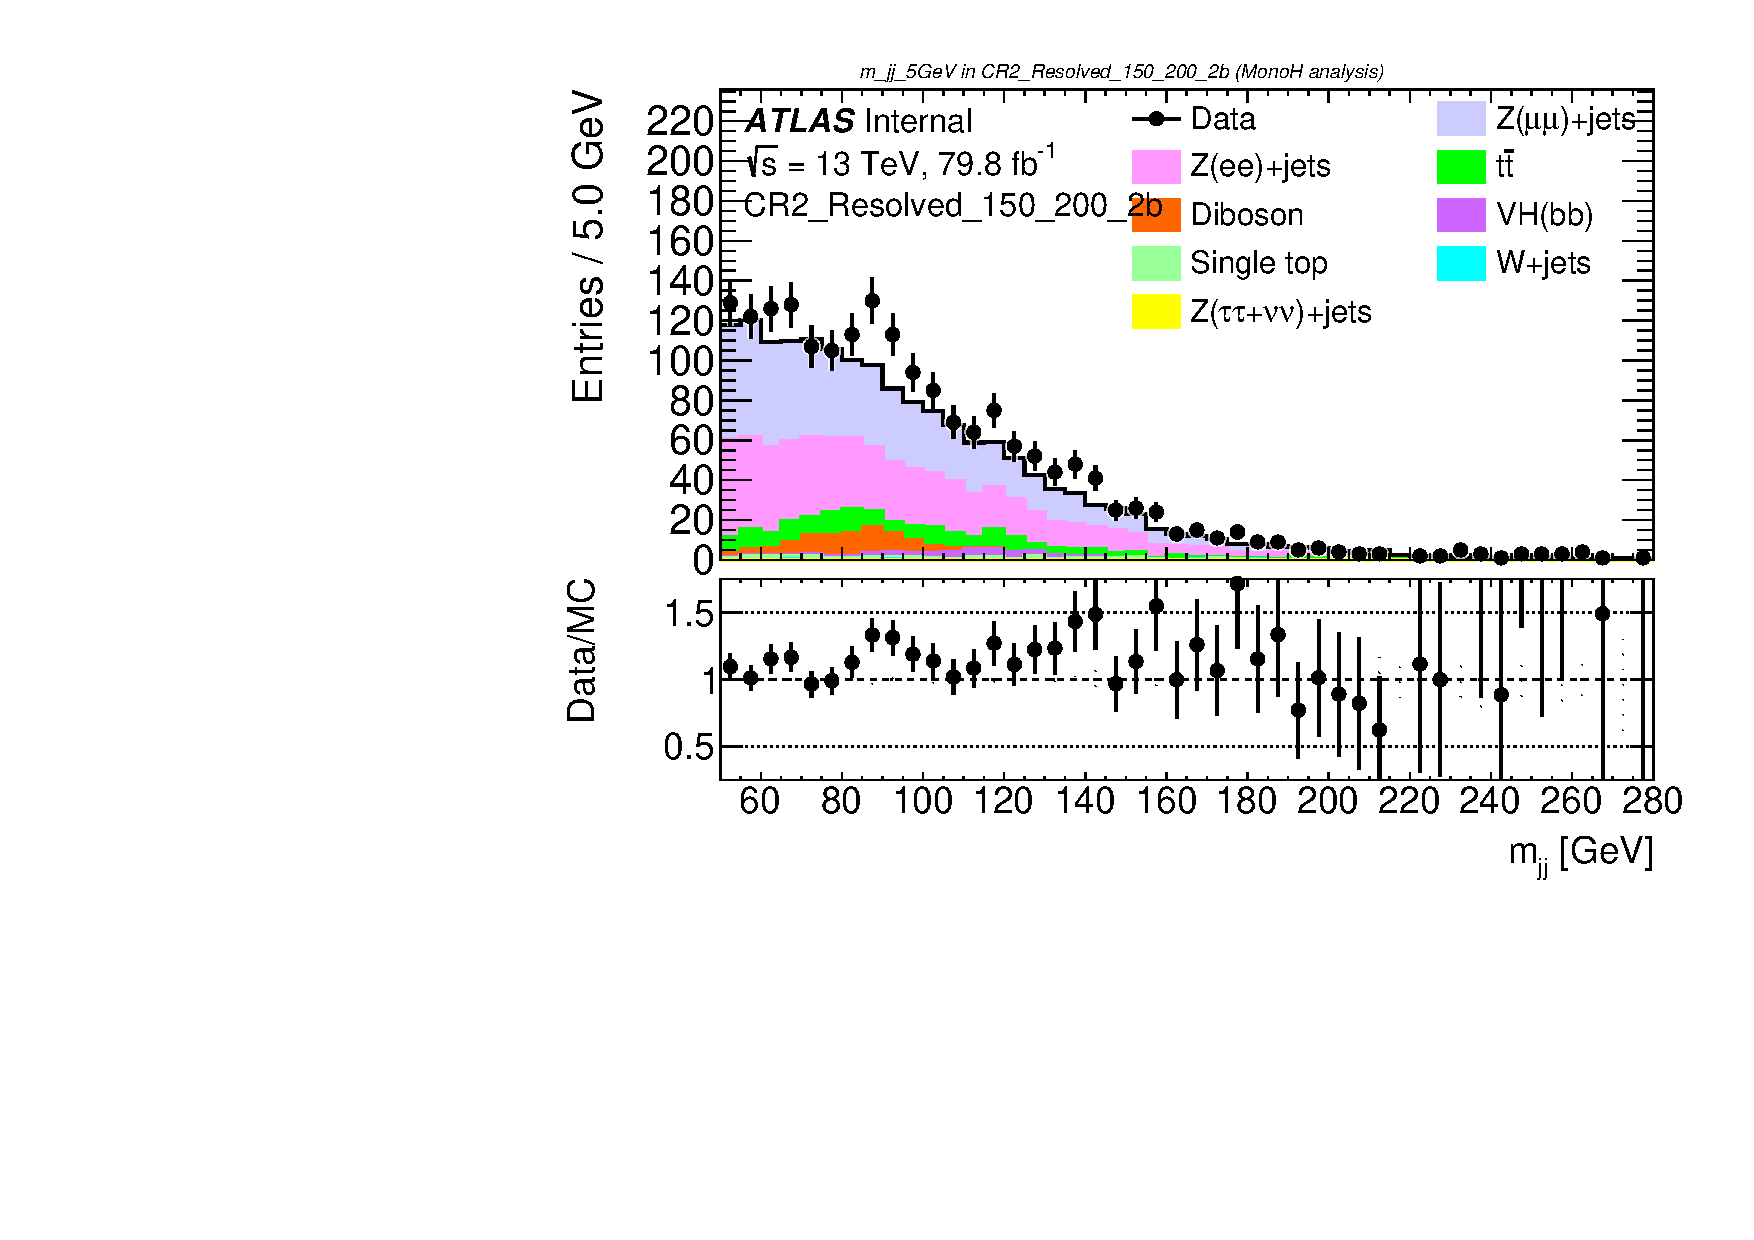
\includegraphics[width=0.47\linewidth]{prefit-150-200.pdf}}
	\subcaptionbox
		{$200\, \mathrm{GeV} < p^V_T < 350\, \mathrm{GeV}$
		\label{fig:2-lep-prefit-fig2}}
		{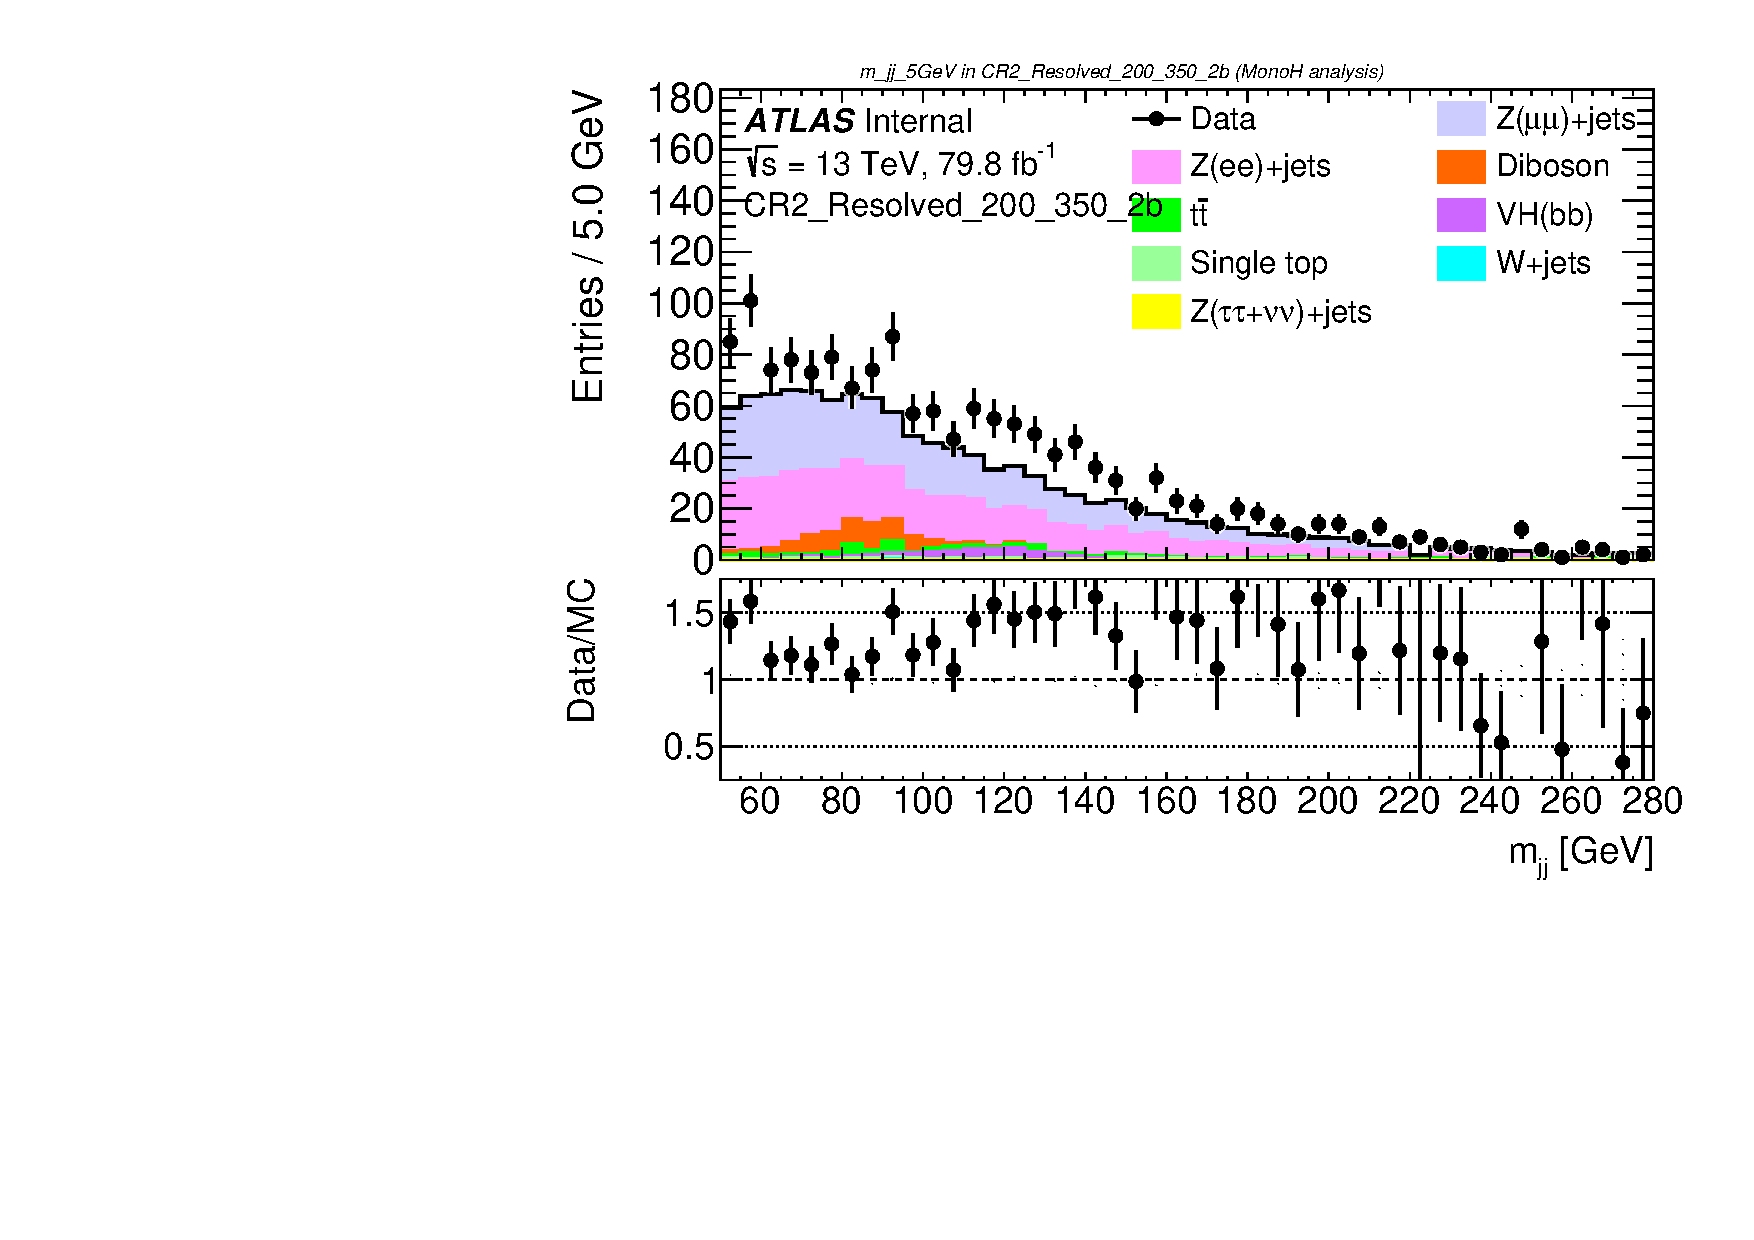
\includegraphics[width=0.47\linewidth]{prefit-200-350.pdf}}
	\vspace{\baselineskip}
	\subcaptionbox
		{$350\, \mathrm{GeV} < p^V_T < 500\, \mathrm{GeV}$
		\label{fig:2-lep-prefit-fig3}}
		{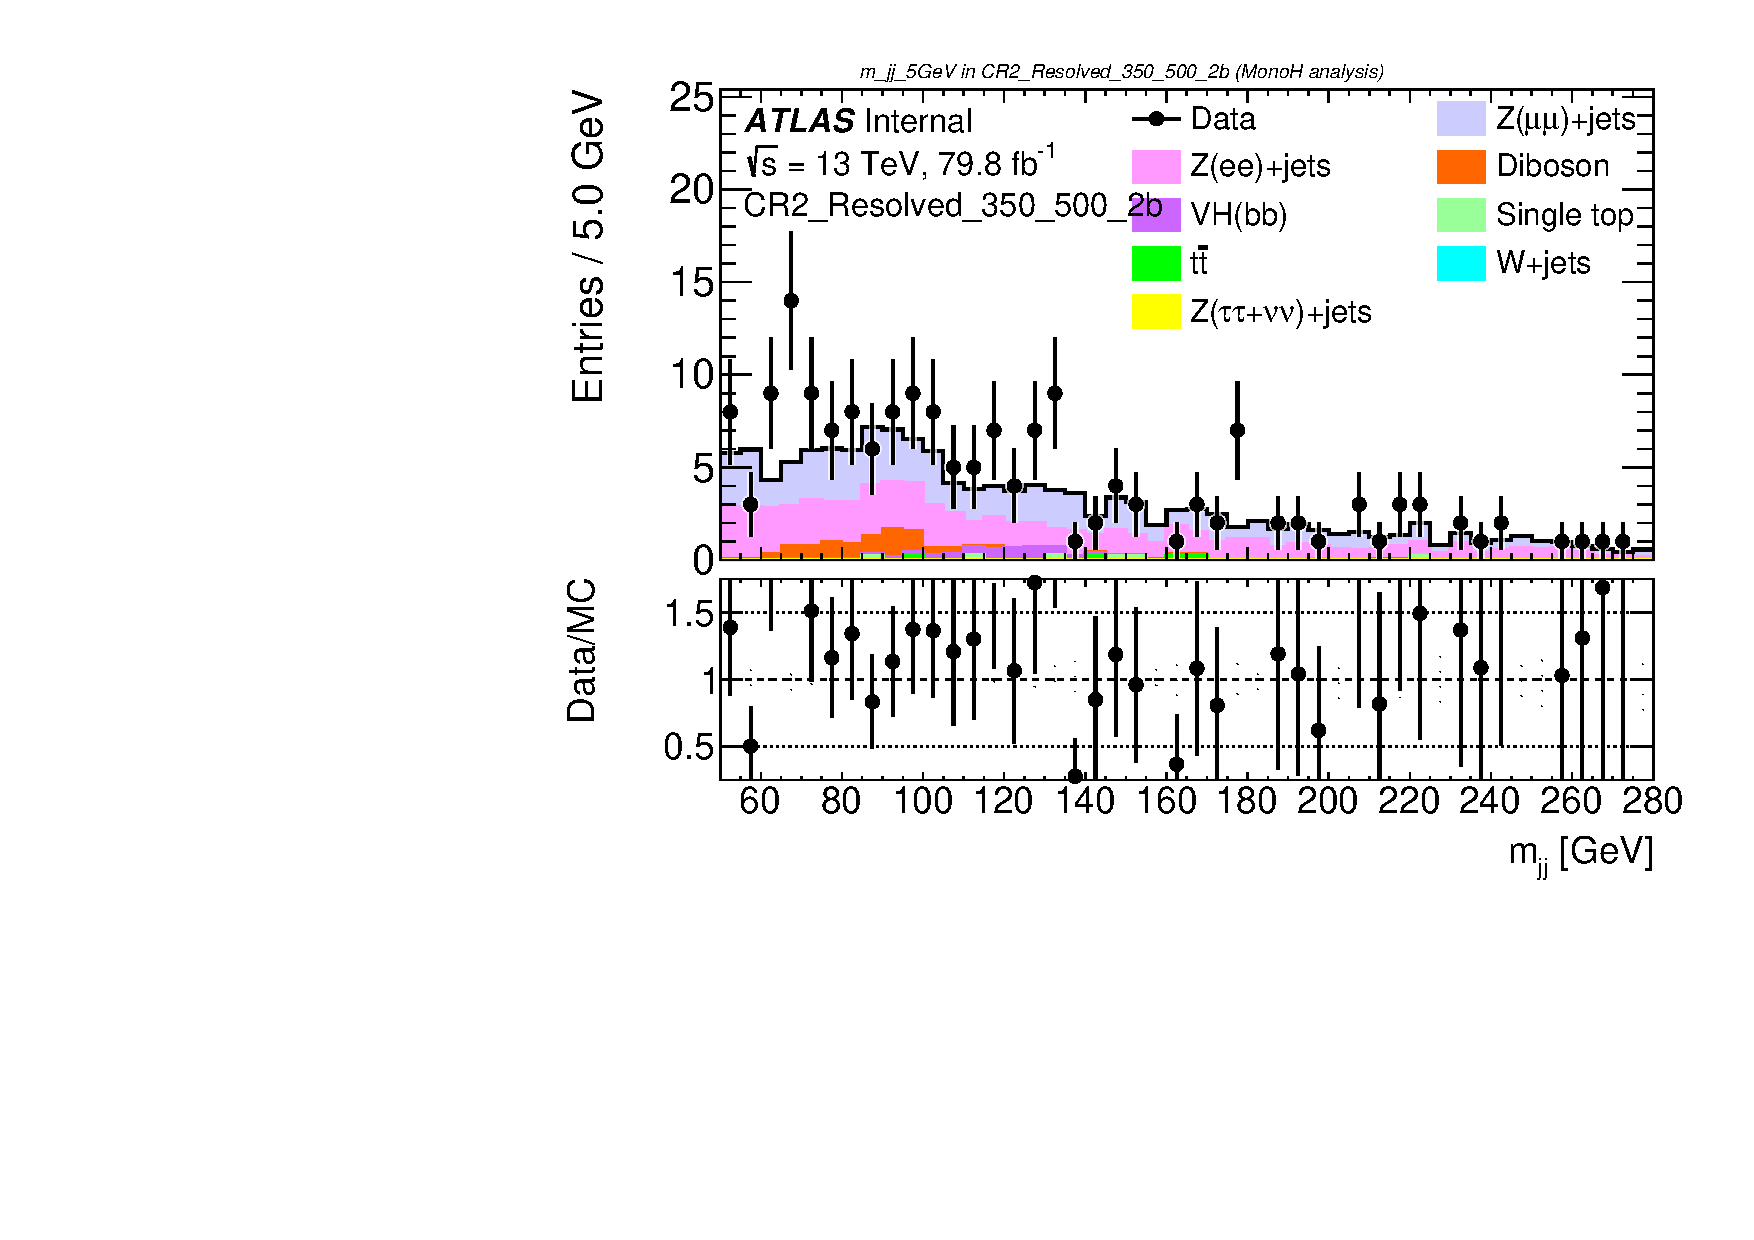
\includegraphics[width=0.47\linewidth]{prefit-350-500.pdf}}
	\subcaptionbox
		{$p^V_T > 500\, \mathrm{GeV}$
		\label{fig:2-lep-prefit-fig4}}
		{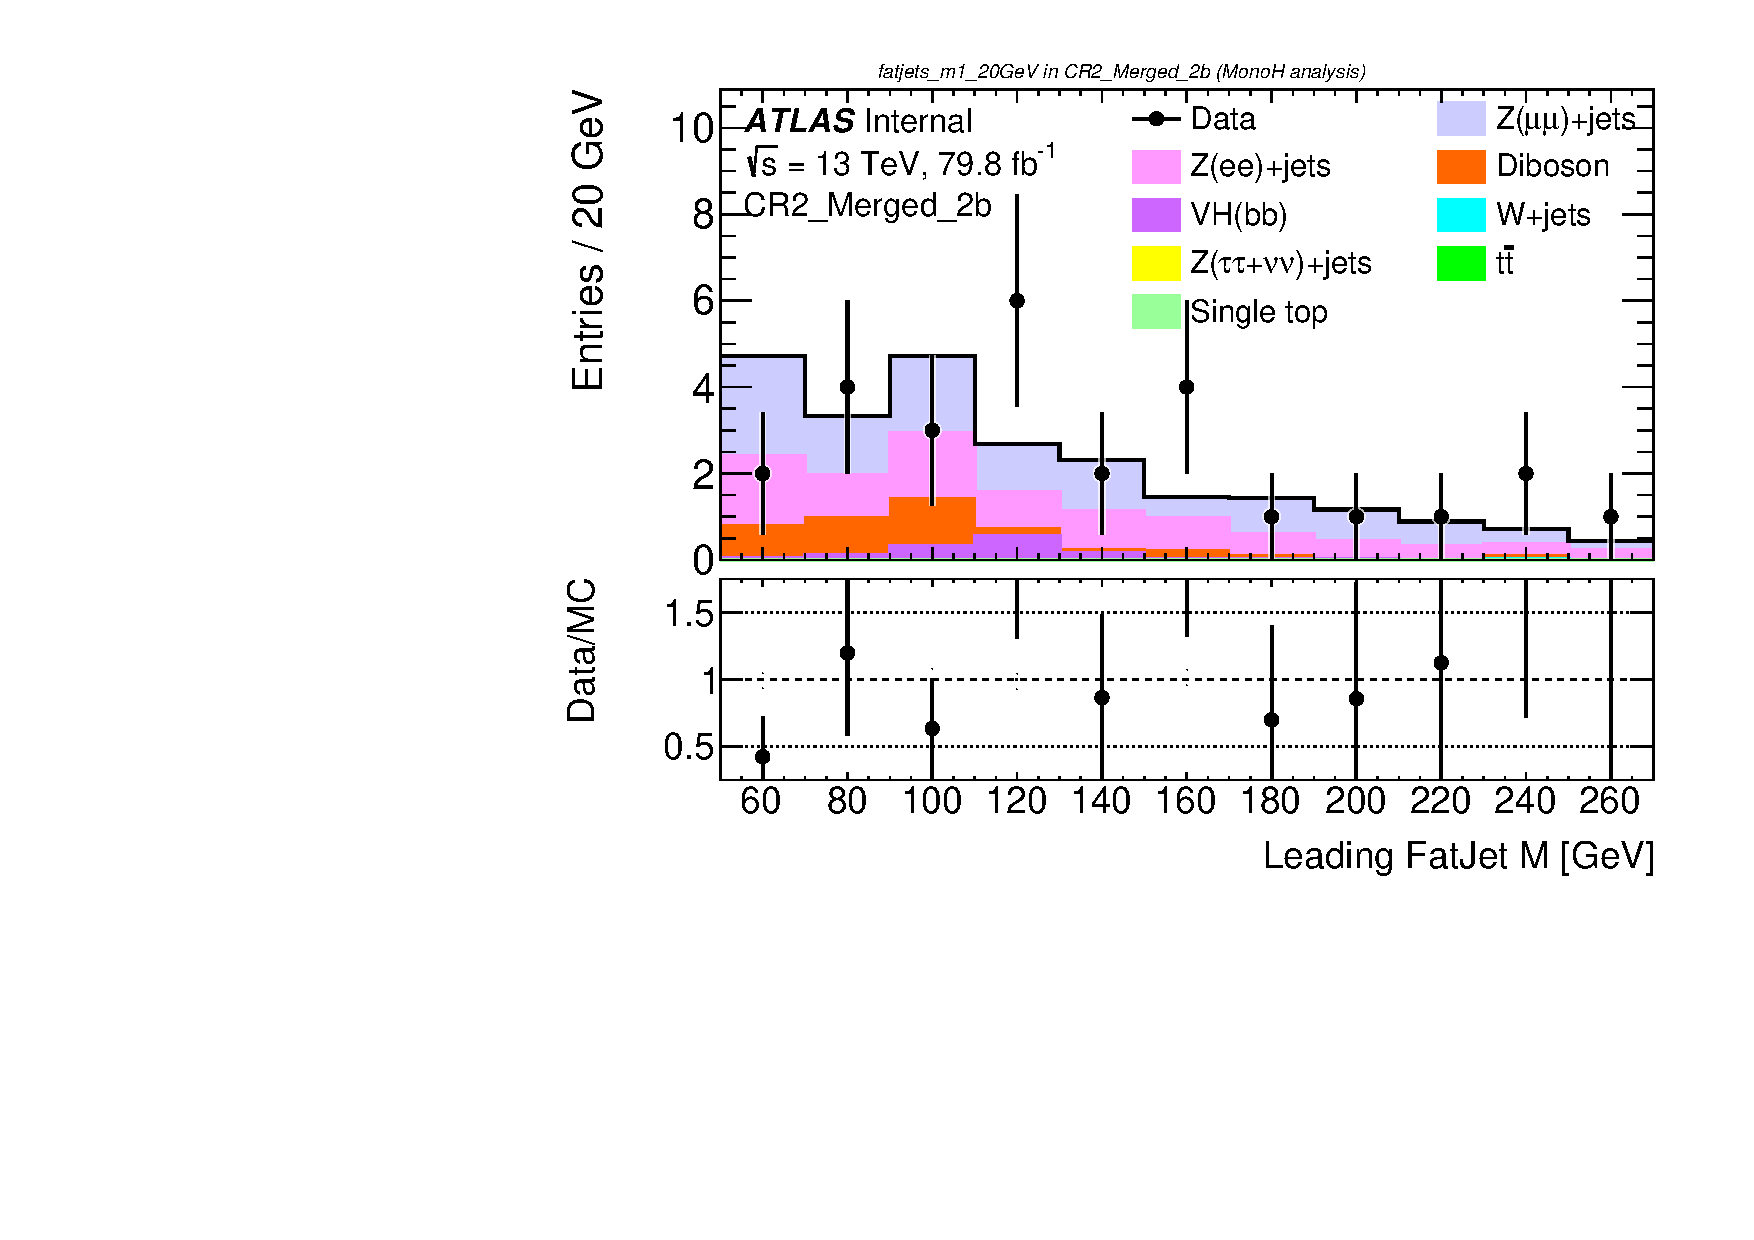
\includegraphics[width=0.47\linewidth]{prefit-500.pdf}}
	\caption{The pre-fit data/MC comparison of $m_{bb}$ distribution. The plots are split into four $p^V_T$ regions for fitting.}
	\label{fig:2-lep-prefit}
\end{figure}

The MC is compared to the data for the distribution for deriving the shape uncertainty in the two-lepton CR. Due to the high purity, the data-driven shape comparison is used for the estimation of the systematic uncertainty on the theoretical prediction of the $Z$ + jets modeling. The shape uncertainty is extracted by following the previous $VH$($bb$) analysis \cite{ATLAS-CONF-2018-036} and is used for two variables, $m_{bb}$ and $p^V_T$. To check if the functions can still give a reasonable estimation, the shape uncertainty and the normalized distribution of $m_{bb}$ and $p^V_T$ are shown in \Cref{fig:shape-uncertainty}. The distributions of the two variables are normalized and compared. The derived functions representing the shape uncertainty on $p^V_T$ and $m_{bb}$ are $\pm 0.2\, \mathrm{log}_{10} (p^V_T/50\, \mathrm{GeV})$ and $\pm 0.0005 (m_{jj} - 100\, \mathrm{GeV})$.

\begin{figure}[!hbt]
	% \captionsetup[subfigure]{labelformat=empty}
	\centering
	\subcaptionbox
	{The distribution of $m_{bb}$.
		\label{fig:shape-uncertainty-fig1}}
		{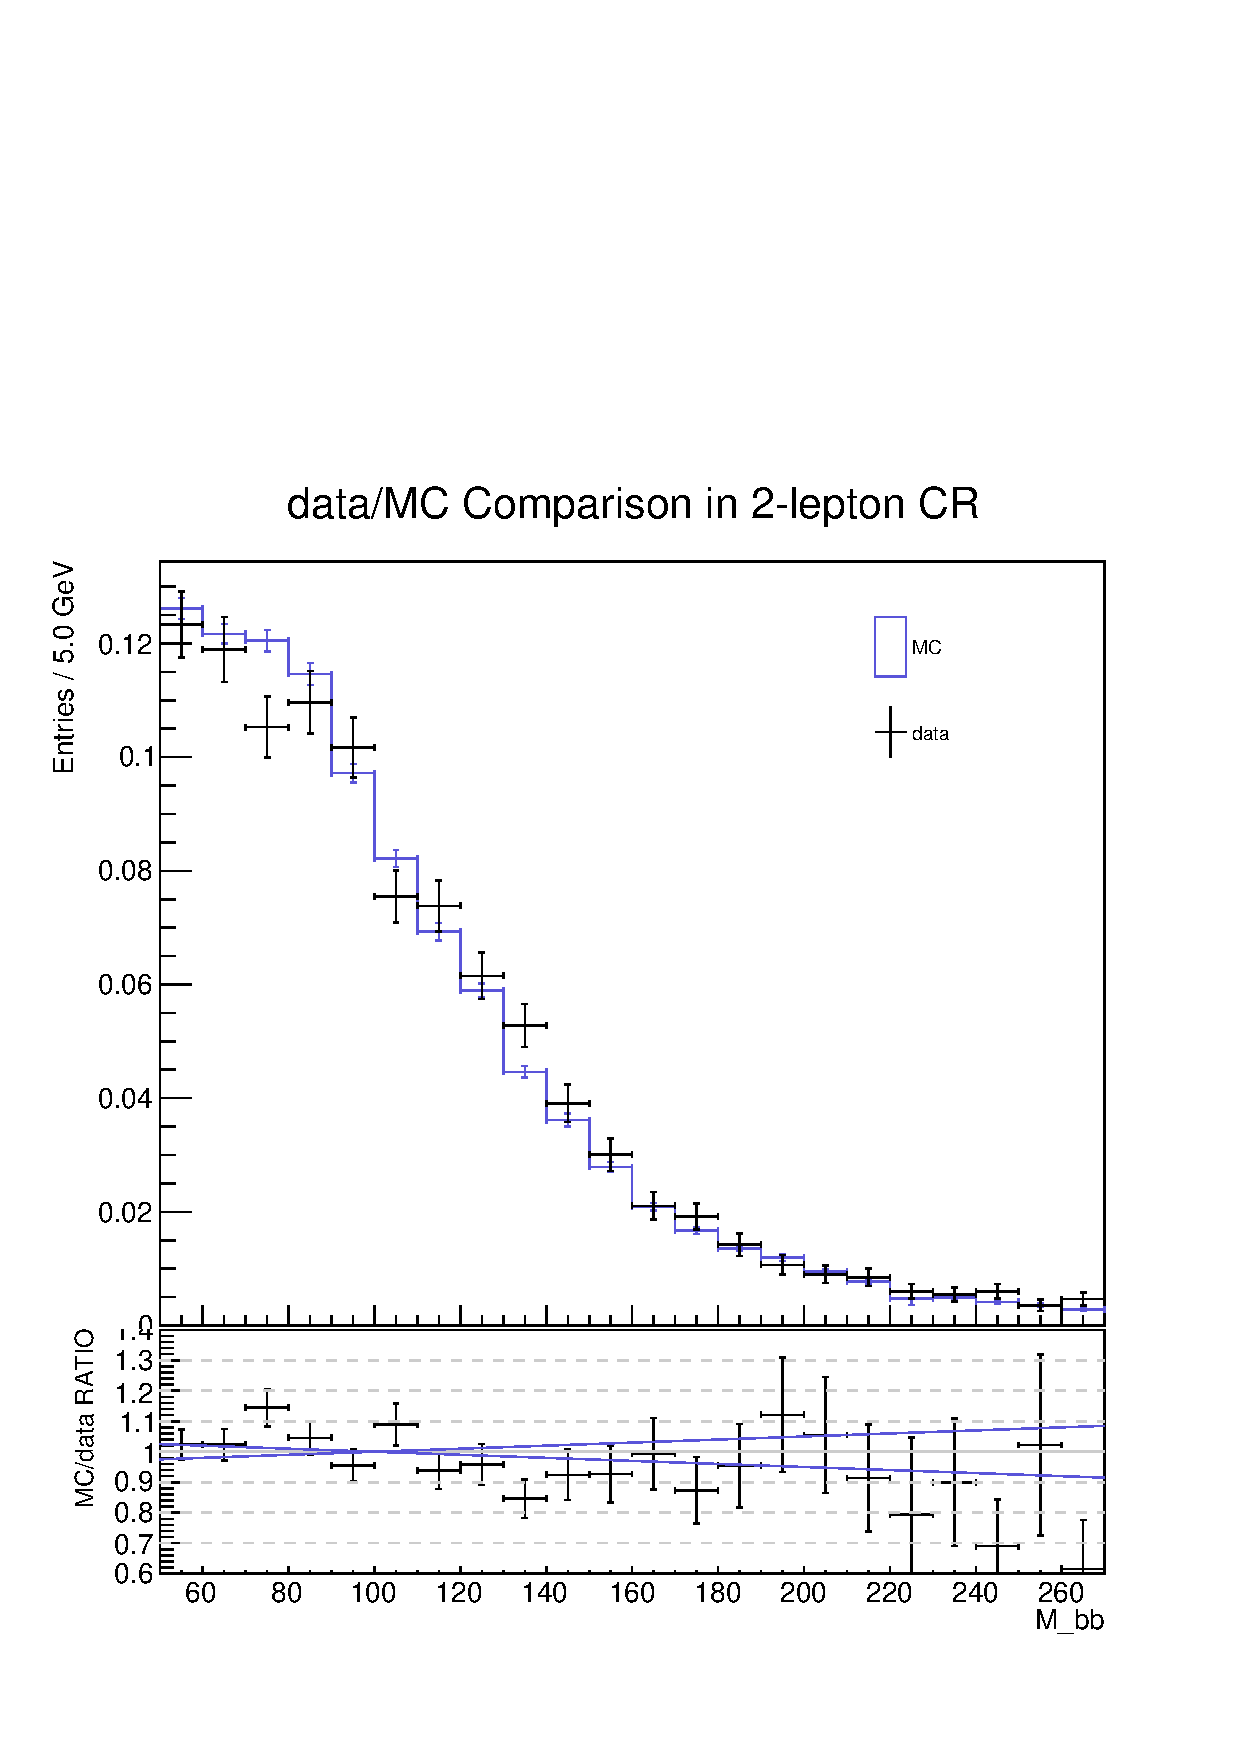
\includegraphics[width=0.65\linewidth]{shape-uncertainty-Mbb.pdf}}
	\vspace{\baselineskip}
	\subcaptionbox
	{The distribution of $p^V_T$.
		\label{fig:shape-uncertainty-fig2}}
		{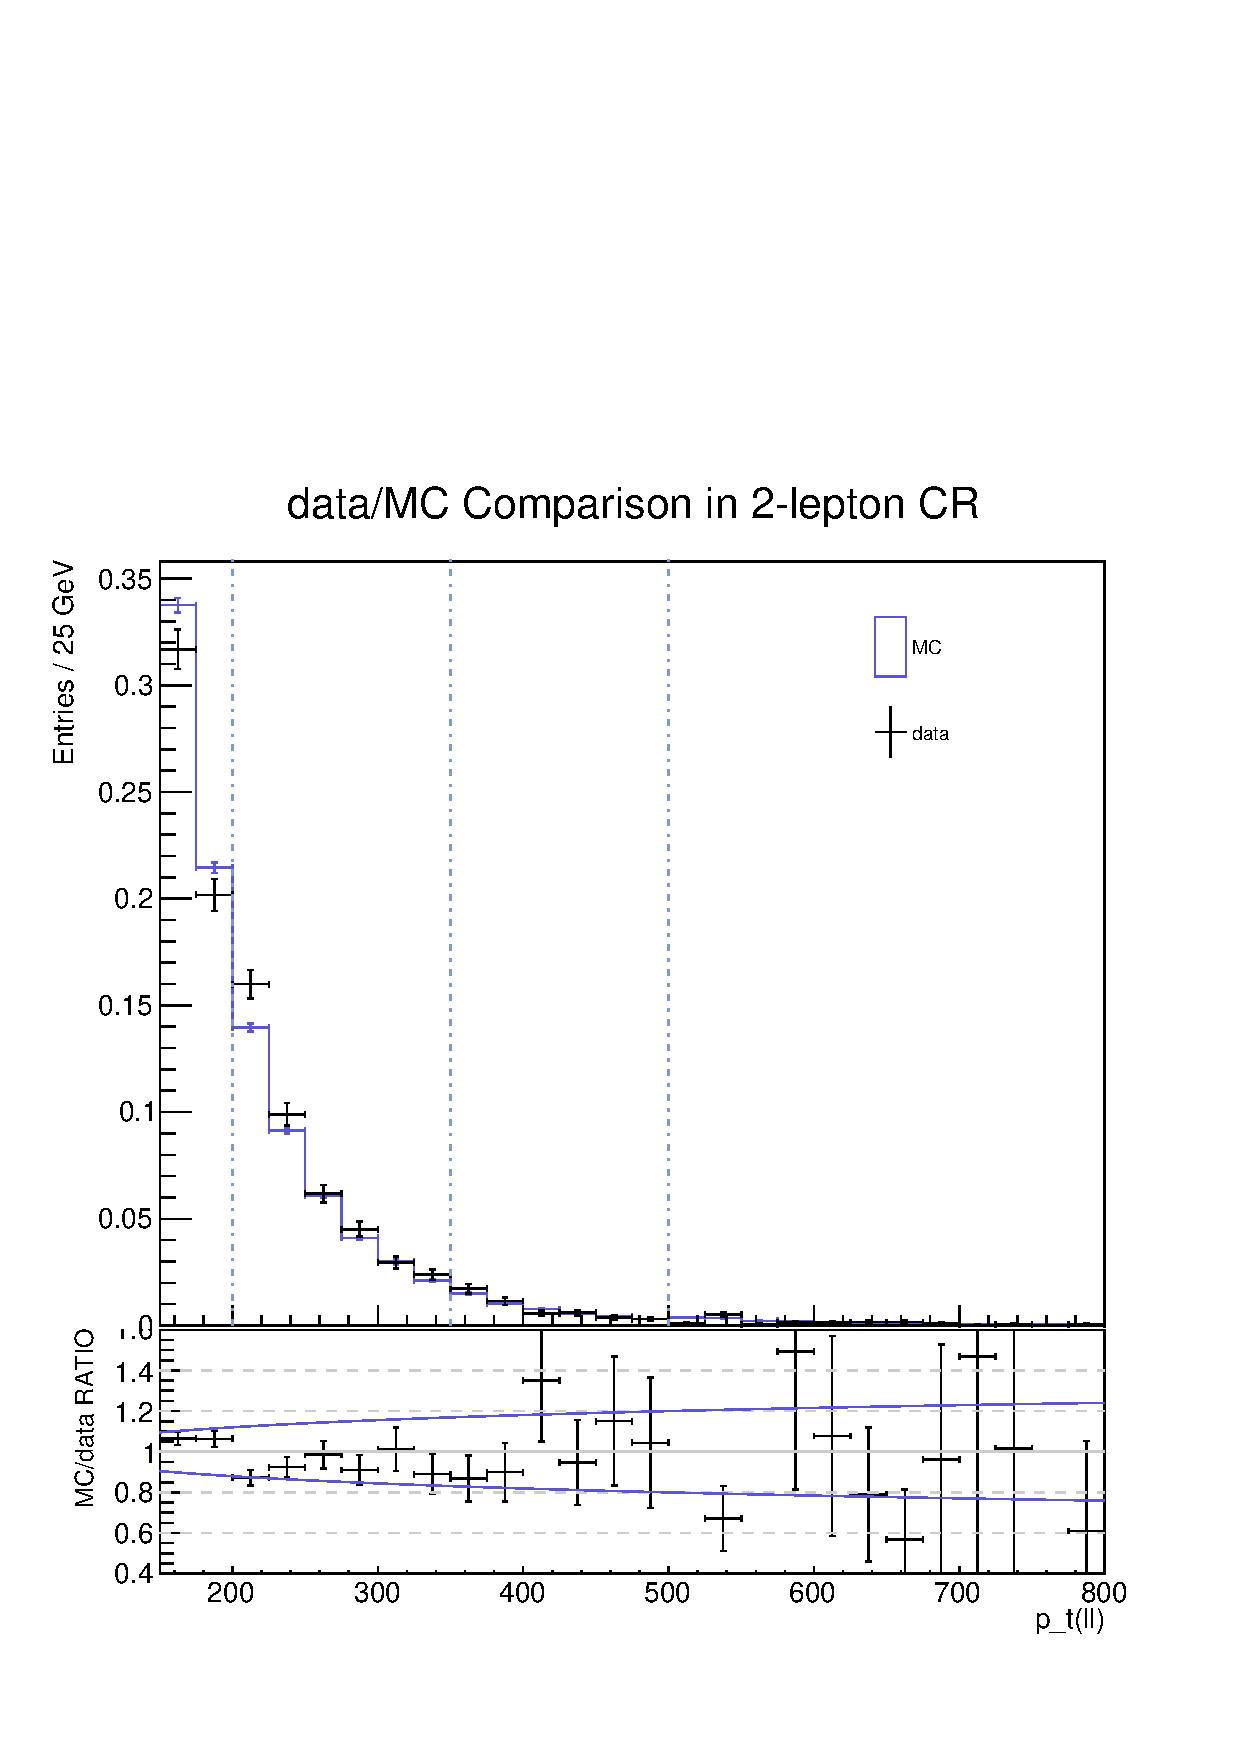
\includegraphics[width=0.65\linewidth]{shape-uncertainty-PTV.pdf}}
	\caption{The shape uncertainties and the normalized distributions of (a) $m_{bb}$ and (b) $p^V_T$. The shape uncertainties are derived by the $VH$($bb$) analysis and gives a reasonable estimation.}
	\label{fig:shape-uncertainty}
\end{figure}

To extrapolate the $Z$ + jets from the two-lepton CR to the SR, the distribution of $p^V_T$ of the $Z$($ll$) + jets and the $Z$($\nu\nu$) + jets are compared in \Cref{fig:Zvv-vs-Zll}. An uncertainty is applied as the decorrelation in the SR due to the larger purity of the $Z$ + jets prediction in the two-lepton CR. This uncertainty is set to be 7\% by following the $VH$($bb$) analysis \cite{ATLAS-CONF-2018-036} and gives a reasonable estimation in the resolved region. For the merged region, this uncertainty doesn't work so well because the merged region concept is not used in the $VH$($bb$) analysis. In the end, the post-fit results are presented in \Cref{fig:2-lep-postfit}. The normalization factor is extracted in the fit and used for the $Z$($\nu\nu$) + jets background in the SR, which is described in the \Cref{chap:result}.

\fig[0.65][fig:Zvv-vs-Zll][!hbt]{Zvv-vs-Zll.pdf}[The comparison of the normalized distributions of the $Z$($ll$) + jets and the $Z$($\nu\nu$) + jets. The uncertainty of the extrapolation from the two-lepton CR to the SR is 7\%, derived by the previous $VH$($bb$) analysis.]

\begin{figure}[!hbt]
	\captionsetup[subfigure]{labelformat=empty}
	\centering
	\subcaptionbox
	{$150\, \mathrm{GeV} < p^V_T < 200\, \mathrm{GeV}$
		\label{fig:2-lep-postfit-fig1}}
		{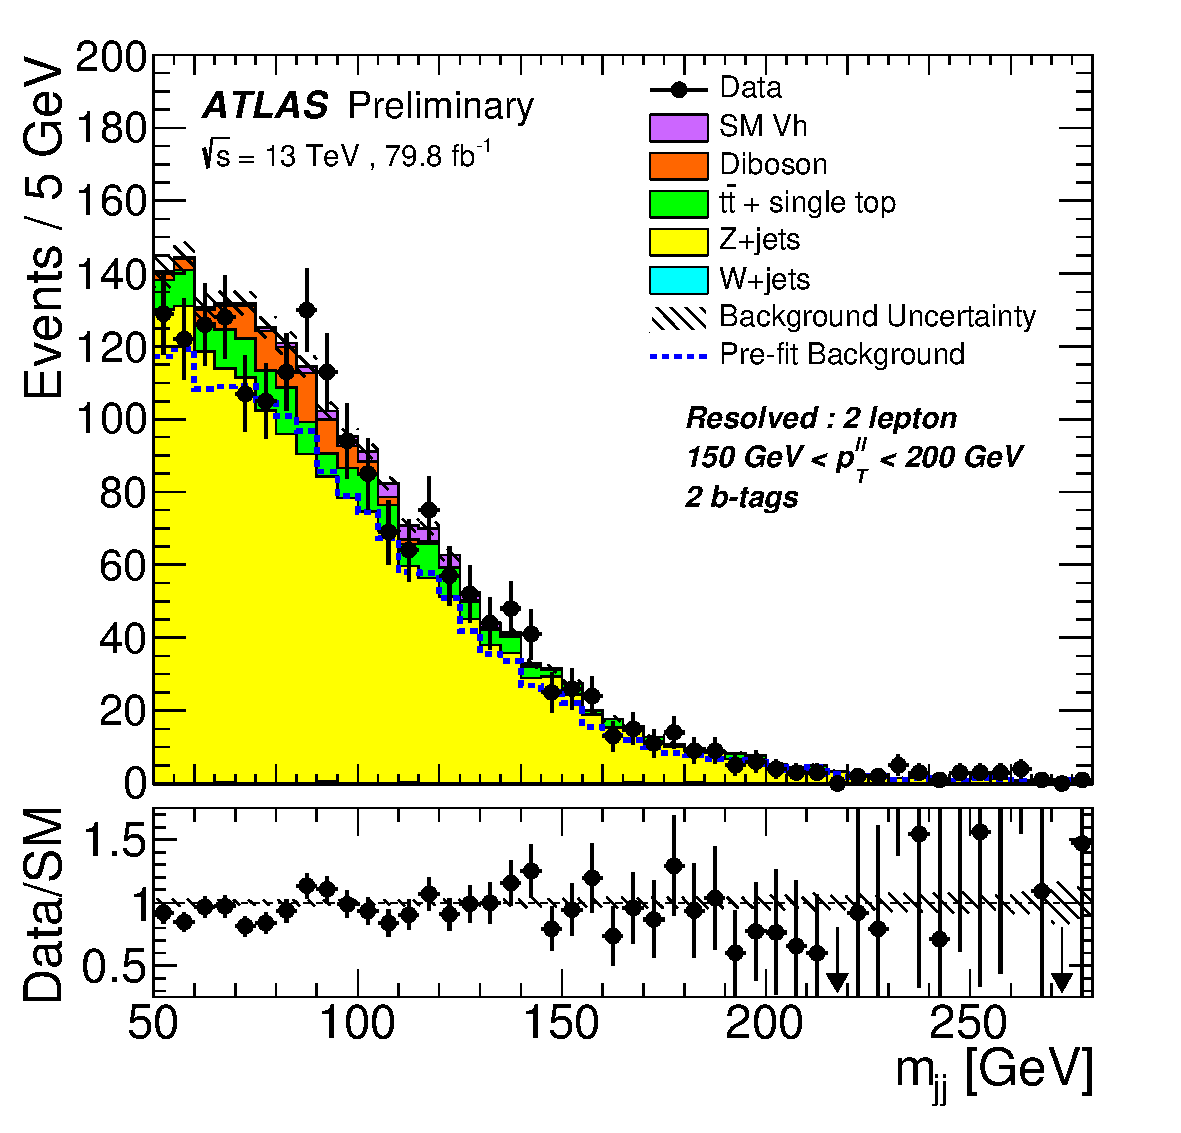
\includegraphics[width=0.47\linewidth]{postfit-150-200.pdf}}
	\subcaptionbox
	{$200\, \mathrm{GeV} < p^V_T < 350\, \mathrm{GeV}$
		\label{fig:2-lep-postfit-fig2}}
		{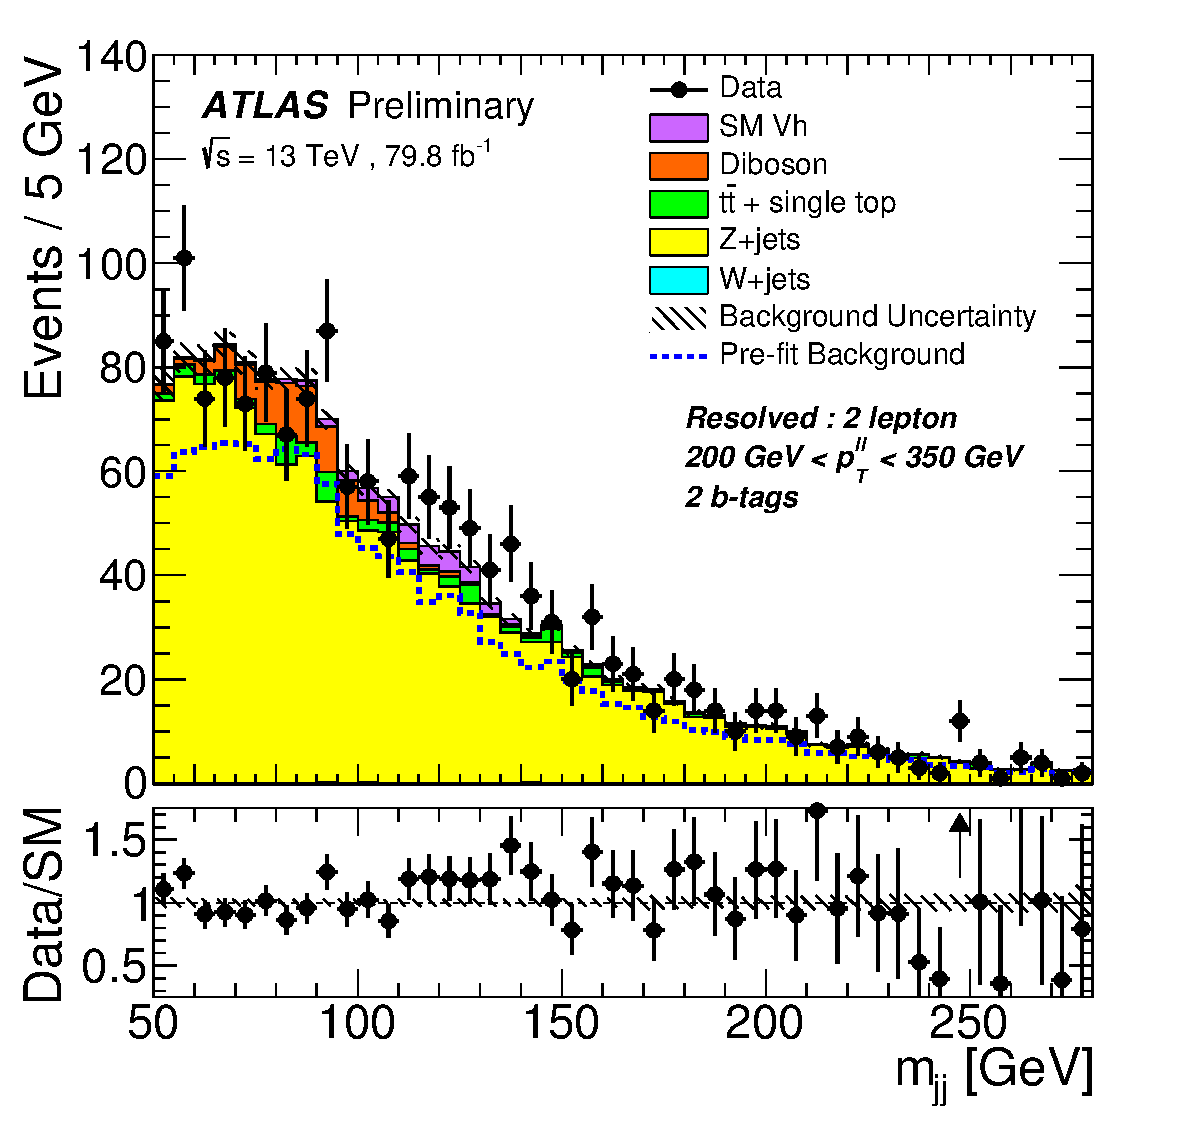
\includegraphics[width=0.47\linewidth]{postfit-200-350.pdf}}
	\vspace{\baselineskip}
	\subcaptionbox
	{$350\, \mathrm{GeV} < p^V_T < 500\, \mathrm{GeV}$
		\label{fig:2-lep-postfit-fig3}}
		{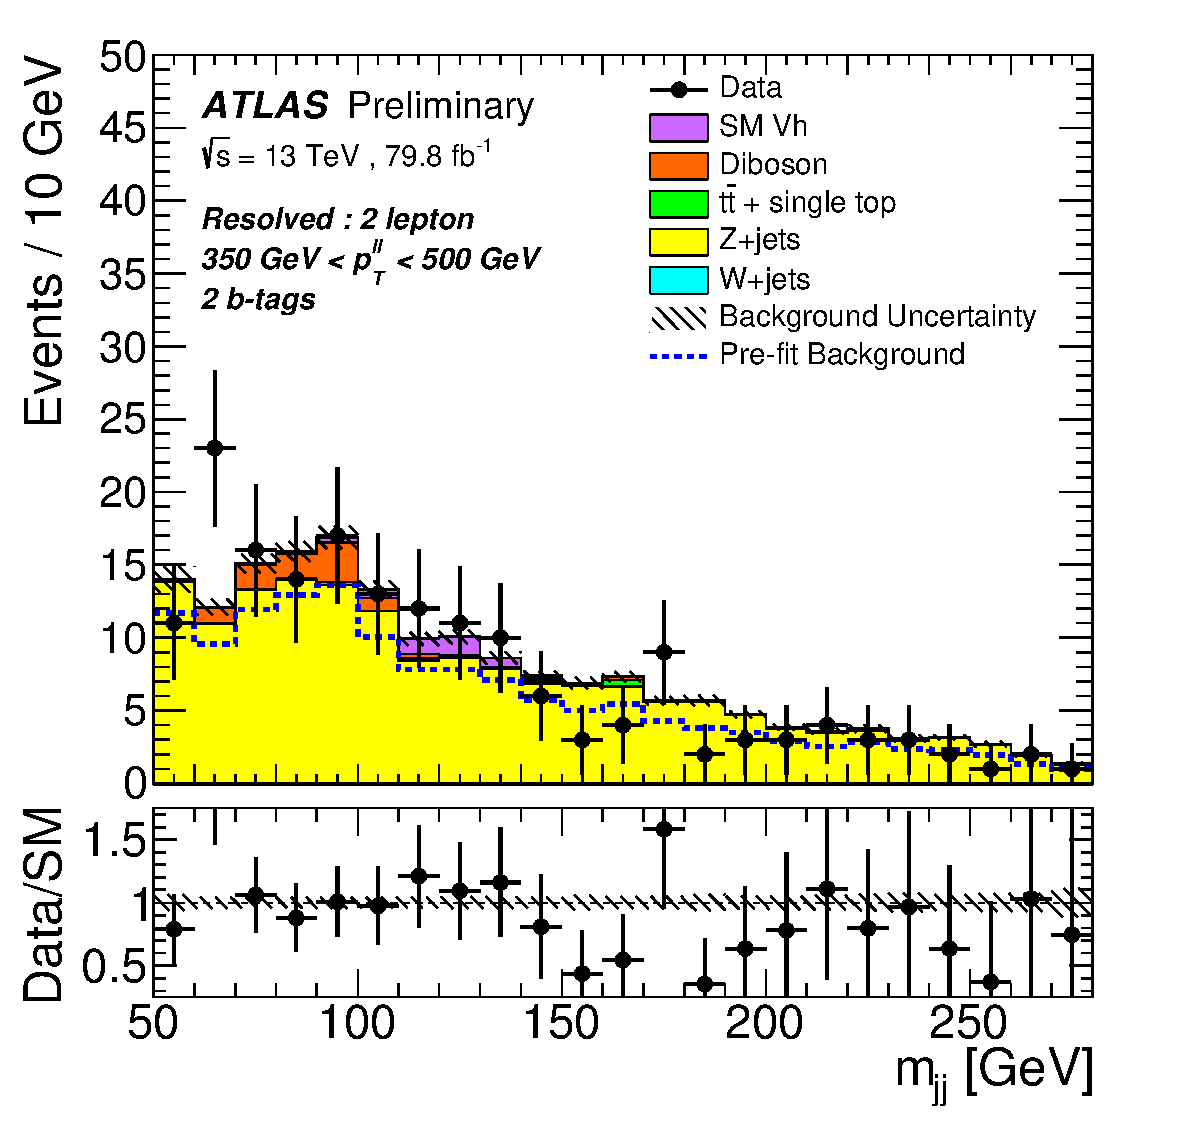
\includegraphics[width=0.47\linewidth]{postfit-350-500.pdf}}
	\subcaptionbox
	{$p^V_T > 500\, \mathrm{GeV}$
		\label{fig:2-lep-postfit-fig4}}
		{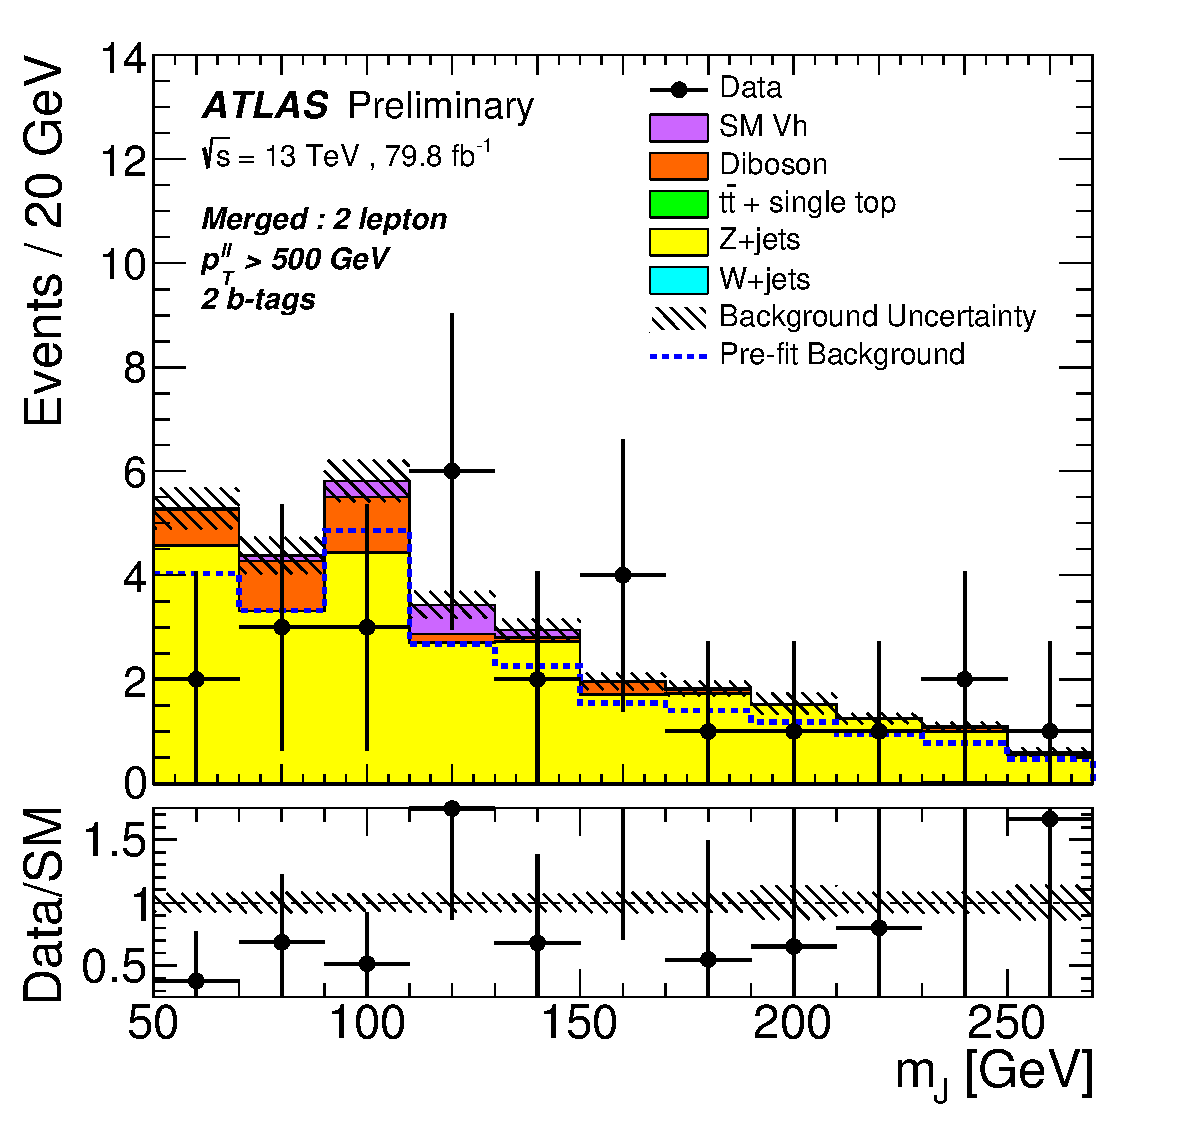
\includegraphics[width=0.47\linewidth]{postfit-500.pdf}}
	\caption{The post-fit data/MC comparison of $m_{bb}$ distribution. The plots are split into four $p^V_T$ regions for fitting.}
	\label{fig:2-lep-postfit}
\end{figure}

\end{document}